\pagebreak
\chapter{Arbeitsaufwand}



\begin{figure}[htbp]
	\begin{minipage}{0.5\textwidth} 
Bei 12 ECTS Punkten für die Bachelorarbeit, ist ein Total von 720 Stunden vorgesehen (12*30h = 360h pro Person). Effektiv wurden total 758 Stunden aufgewendet. Daraus ergibt sich ein Mehraufwand von 38 Stunden.
	\end{minipage}
	\hfill
	\begin{minipage}{0.45\textwidth}
		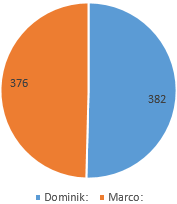
\includegraphics[scale=0.65]{appendix/img/aufwand1}
		\caption{Aufwand Total}
		\label{fig:aufwand1}
	\end{minipage}
\end{figure}

\begin{figure}[htbp]
	\begin{minipage}{0.5\textwidth} 
Die Abbildung \ref{fig:aufwand2} zeigt den Aufwand in Stunden pro Phase. Daraus sieht man, dass in die letzte Construction-Phase (C3) am meisten Aufwand investiert wurde.
	\end{minipage}
	\hfill
	\begin{minipage}{0.45\textwidth}
		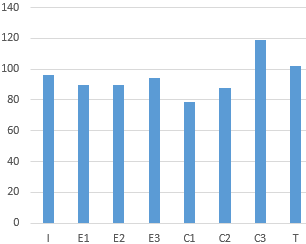
\includegraphics[scale=0.65]{appendix/img/aufwand2}
		\caption{Aufwand nach Phase}
		\label{fig:aufwand2}
	\end{minipage}
\end{figure}

\begin{figure}[htbp]
	\begin{minipage}{0.5\textwidth} 
Mit 52\% stellt die Implementation die grösste Tätigkeit dar. Für die Dokumentation und die Analyse wurde gleichermassen viel Aufwand geleistet. Am wenigsten wurde in die Administration investiert, da in dieser Tätigkeit am Meisten am Projektplan gearbeitet wurde, der in der ersten Phase erstellt wurde.
	\end{minipage}
	\hfill
	\begin{minipage}{0.45\textwidth}
		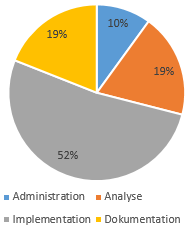
\includegraphics[scale=0.65]{appendix/img/aufwand3}
		\caption{Aufwand nach Tätigkeit}
		\label{fig:aufwand3}
	\end{minipage}
\end{figure}